%-----------------------------------------------------------------------------------------------------------------------------------------------%
%	The MIT License (MIT)
%
%	Copyright (c) 2021 Jitin Nair
%
%	Permission is hereby granted, free of charge, to any person obtaining a copy
%	of this software and associated documentation files (the "Software"), to deal
%	in the Software without restriction, including without limitation the rights
%	to use, copy, modify, merge, publish, distribute, sublicense, and/or sell
%	copies of the Software, and to permit persons to whom the Software is
%	furnished to do so, subject to the following conditions:
%	
%	THE SOFTWARE IS PROVIDED "AS IS", WITHOUT WARRANTY OF ANY KIND, EXPRESS OR
%	IMPLIED, INCLUDING BUT NOT LIMITED TO THE WARRANTIES OF MERCHANTABILITY,
%	FITNESS FOR A PARTICULAR PURPOSE AND NONINFRINGEMENT. IN NO EVENT SHALL THE
%	AUTHORS OR COPYRIGHT HOLDERS BE LIABLE FOR ANY CLAIM, DAMAGES OR OTHER
%	LIABILITY, WHETHER IN AN ACTION OF CONTRACT, TORT OR OTHERWISE, ARISING FROM,
%	OUT OF OR IN CONNECTION WITH THE SOFTWARE OR THE USE OR OTHER DEALINGS IN
%	THE SOFTWARE.
%	
%
%-----------------------------------------------------------------------------------------------------------------------------------------------%

%----------------------------------------------------------------------------------------
%	DOCUMENT DEFINITION
%----------------------------------------------------------------------------------------

% article class because we want to fully customize the page and not use a cv template
\documentclass[a4paper,12pt]{article}

%----------------------------------------------------------------------------------------
%	FONT
%----------------------------------------------------------------------------------------

% % fontspec allows you to use TTF/OTF fonts directly
% \usepackage{fontspec}
% \defaultfontfeatures{Ligatures=TeX}

% % modified for ShareLaTeX use
% \setmainfont[
% SmallCapsFont = Fontin-SmallCaps.otf,
% BoldFont = Fontin-Bold.otf,
% ItalicFont = Fontin-Italic.otf
% ]
% {Fontin.otf}

%----------------------------------------------------------------------------------------
%	PACKAGES
%----------------------------------------------------------------------------------------
\usepackage{url}
\usepackage{parskip} 	

%other packages for formatting
\RequirePackage{color}
\RequirePackage{graphicx}
\usepackage[usenames,dvipsnames]{xcolor}
\usepackage[scale=0.9]{geometry}

%tabularx environment
\usepackage{tabularx}

%for lists within experience section
\usepackage{enumitem}

% centered version of 'X' col. type
\newcolumntype{C}{>{\centering\arraybackslash}X} 

%to prevent spillover of tabular into next pages
\usepackage{supertabular}
\usepackage{tabularx}
\newlength{\fullcollw}
\setlength{\fullcollw}{0.47\textwidth}

%custom \section
\usepackage{titlesec}				
\usepackage{multicol}
\usepackage{multirow}

%CV Sections inspired by: 
%http://stefano.italians.nl/archives/26
\titleformat{\section}{\Large\scshape\raggedright}{}{0em}{}[\titlerule]
\titlespacing{\section}{0pt}{10pt}{10pt}

%for publications
\usepackage[style=authoryear,sorting=ynt, maxbibnames=2]{biblatex}

%Setup hyperref package, and colours for links
\usepackage[unicode, draft=false]{hyperref}
\definecolor{linkcolour}{rgb}{0,0.2,0.6}
\hypersetup{colorlinks,breaklinks,urlcolor=linkcolour,linkcolor=linkcolour}
\addbibresource{citations.bib}
\setlength\bibitemsep{1em}

%for social icons
\usepackage{fontawesome5}

\usepackage{pdfpages}


%debug page outer frames
%\usepackage{showframe}


% job listing environments
\newenvironment{jobshort}[2]
    {
    \begin{tabularx}{\linewidth}{@{}l X r@{}}
    \textbf{#1} & \hfill &  #2 \\[3.75pt]
    \end{tabularx}
    }
    {
    }

\newenvironment{joblong}[2]
    {
    \begin{tabularx}{\linewidth}{@{}l X r@{}}
    \textbf{#1} & \hfill &  #2 \\[3.75pt]
    \end{tabularx}
    \begin{minipage}[t]{\linewidth}
    \begin{itemize}[nosep,after=\strut, leftmargin=1em, itemsep=3pt,label=--]
    }
    {
    \end{itemize}
    \end{minipage}    
    }



%----------------------------------------------------------------------------------------
%	BEGIN DOCUMENT
%----------------------------------------------------------------------------------------
\begin{document}

% non-numbered pages
\pagestyle{empty} 

%----------------------------------------------------------------------------------------
%	TITLE
%----------------------------------------------------------------------------------------

% \begin{tabularx}{\linewidth}{ @{}X X@{} }
% \huge{Your Name}\vspace{2pt} & \hfill \emoji{incoming-envelope} email@email.com \\
% \raisebox{-0.05\height}\faGithub\ username \ | \
% \raisebox{-0.00\height}\faLinkedin\ username \ | \ \raisebox{-0.05\height}\faGlobe \ mysite.com  & \hfill \emoji{calling} number
% \end{tabularx}

\begin{tabularx}{\linewidth}{@{} C @{}}
\Huge{Giuseppe Maganuco} \\[7.5pt]
\href{https://github.com/Giuko}{\raisebox{-0.05\height}\faGithub\ Giuko} \ $|$ \ 
\href{https://www.linkedin.com/in/giuseppe-maganuco-9766711b4/}{\raisebox{-0.05\height}\faLinkedin\ giuseppe-maganuco} \ $|$ \ 
\href{https://giuko.github.io/}{\raisebox{-0.05\height}\faGlobe \ giuko.github.io} \ $|$ \ 
\href{mailto:peppecicciomaganuco13@gmail.com}{\raisebox{-0.05\height}\faEnvelope \ peppecicciomaganuco13@gmail.com} \ $|$ \ \\
\href{tel:+39 3980946125}{\raisebox{-0.05\height}\faMobile \ +39 389 094 6125} \\
\end{tabularx}

%----------------------------------------------------------------------------------------
% EXPERIENCE SECTIONS
%----------------------------------------------------------------------------------------

%Interests/ Keywords/ Summary
\section{Summary}
Passionate Computer Engineering student with a strong interest in system embedded, fpga, electronics and OS. Always eager to learn and take on new challenges. 

%Experience
%\section{Work Experience}

%\begin{jobshort}{Designation}{Jan 2021 - present}
%long long line of blah blah that will wrap when the table fills the column width long long line of blah blah that will wrap when the table fills the column width long long line of blah blah that will wrap when the table fills the column width long long line of blah blah that will wrap when the table fills the column width
%\end{jobshort}


%\begin{joblong}{Designation}{Mar 2019 - Jan 2021}
%\item long long line of blah blah that will wrap when the table fills the column width
%\item again, long long line of blah blah that will wrap when the table fills the column width but this time even more long long line of blah blah. again, long long line of blah blah that will wrap when the table fills the column width but this time even more long long line of blah blah
%\end{joblong}
  
%Projects
\section{Projects}
For a better overwiev of the projects done: \href{https://giuko.github.io/}{\raisebox{-0.05\height}\faGlobe \ giuko.github.io} 
\\
\\
%\begin{tabularx}{\linewidth}{ @{}l r@{} }
\begin{tabularx}{\linewidth}{ @{}>{\raggedright\arraybackslash}X r@{} }
\textbf{DLX processor}
\multicolumn{1}{@{}X@{}}{
Full implementation of a pipelined DLX processor architecture in VHDL, a RISC processor with 5 stage (IF, ID, EX, ME, WB). Following the development from the design, simulation, synthesis and physical design. 
}  \\
\end{tabularx}

%\begin{tabularx}{\linewidth}{ @{}l r@{} }
\begin{tabularx}{\linewidth}{ @{}>{\raggedright\arraybackslash}X r@{} }
\textbf{UVM testbench}
\multicolumn{1}{@{}X@{}}{
Development of a UVM testbench in SystemVerilog, written for QuestaSim. Analyzed different possible scenerio, covering: Constrained random test generation, Constrained precise generation, Assertion-based verification, Functional coverage collection and analysis.  
}  \\
\end{tabularx}

%\begin{tabularx}{\linewidth}{ @{}l r@{} }
\begin{tabularx}{\linewidth}{ @{}>{\raggedright\arraybackslash}X r@{} }
\textbf{QEMU Modding}
\multicolumn{1}{@{}X@{}}{
This project involved modifying the QEMU emulator to support the NXP S32K3x8 development board, enabling full system emulation. The work included implementing peripheral emulation, particularly for UART communication, and integrating FreeRTOS support for real-time operating system testing.
}  \\
\end{tabularx}

%\begin{tabularx}{\linewidth}{ @{}l r@{} }
\begin{tabularx}{\linewidth}{ @{}>{\raggedright\arraybackslash}X r@{} }
\textbf{Optimizer for Gate-Level Netlist}
\multicolumn{1}{@{}X@{}}{
Developed a custom power optimization tool written in TCL that analyzes gate-level netlists and optimizes power consumption by intelligently adjusting voltage thresholds of individual cells. The optimizer respects timing and design constraints while maximizing power savings.
}  \\
\end{tabularx}

%----------------------------------------------------------------------------------------
%	EDUCATION
%----------------------------------------------------------------------------------------
\section{Education}
\begin{tabularx}{\linewidth}{@{}l X@{}}	
2024 - present & Master's Degree in Computer Engineering Embedded System - Second year \\

2021 - 2024 & Bachelor's Degree in Computer Engineering, Università di Catania \hfill  (110 cum laude) \\
\end{tabularx}

%----------------------------------------------------------------------------------------
%	PUBLICATIONS
%----------------------------------------------------------------------------------------
%\section{Publications}
%\begin{refsection}[citations.bib]
%\nocite{*}
%\printbibliography[heading=none]
%\end{refsection}

%----------------------------------------------------------------------------------------
%	SKILLS
%----------------------------------------------------------------------------------------
\section{Skills}
\begin{tabularx}{\linewidth}{@{}l X@{}}
Language Spoken & \normalsize{Italian (native), English Fluent (C1 in CEFR)} \\
Hardware Description Language &  \normalsize{VHDL, SystemVerilog}\\
Verification &  \normalsize{UVM}\\
Scripting & \normalsize{Bash, TCL}\\
Tools  &  \normalsize{QEMU, QuestaSIM, Innovus}\\  
Programming Language & \normalsize{C, python}\\
Miscellaneous & \normalsize{FreeRTOS, GIT, Linux, Javascript}
\end{tabularx}

\vfill
\center{\footnotesize Last updated: \today}


\newpage
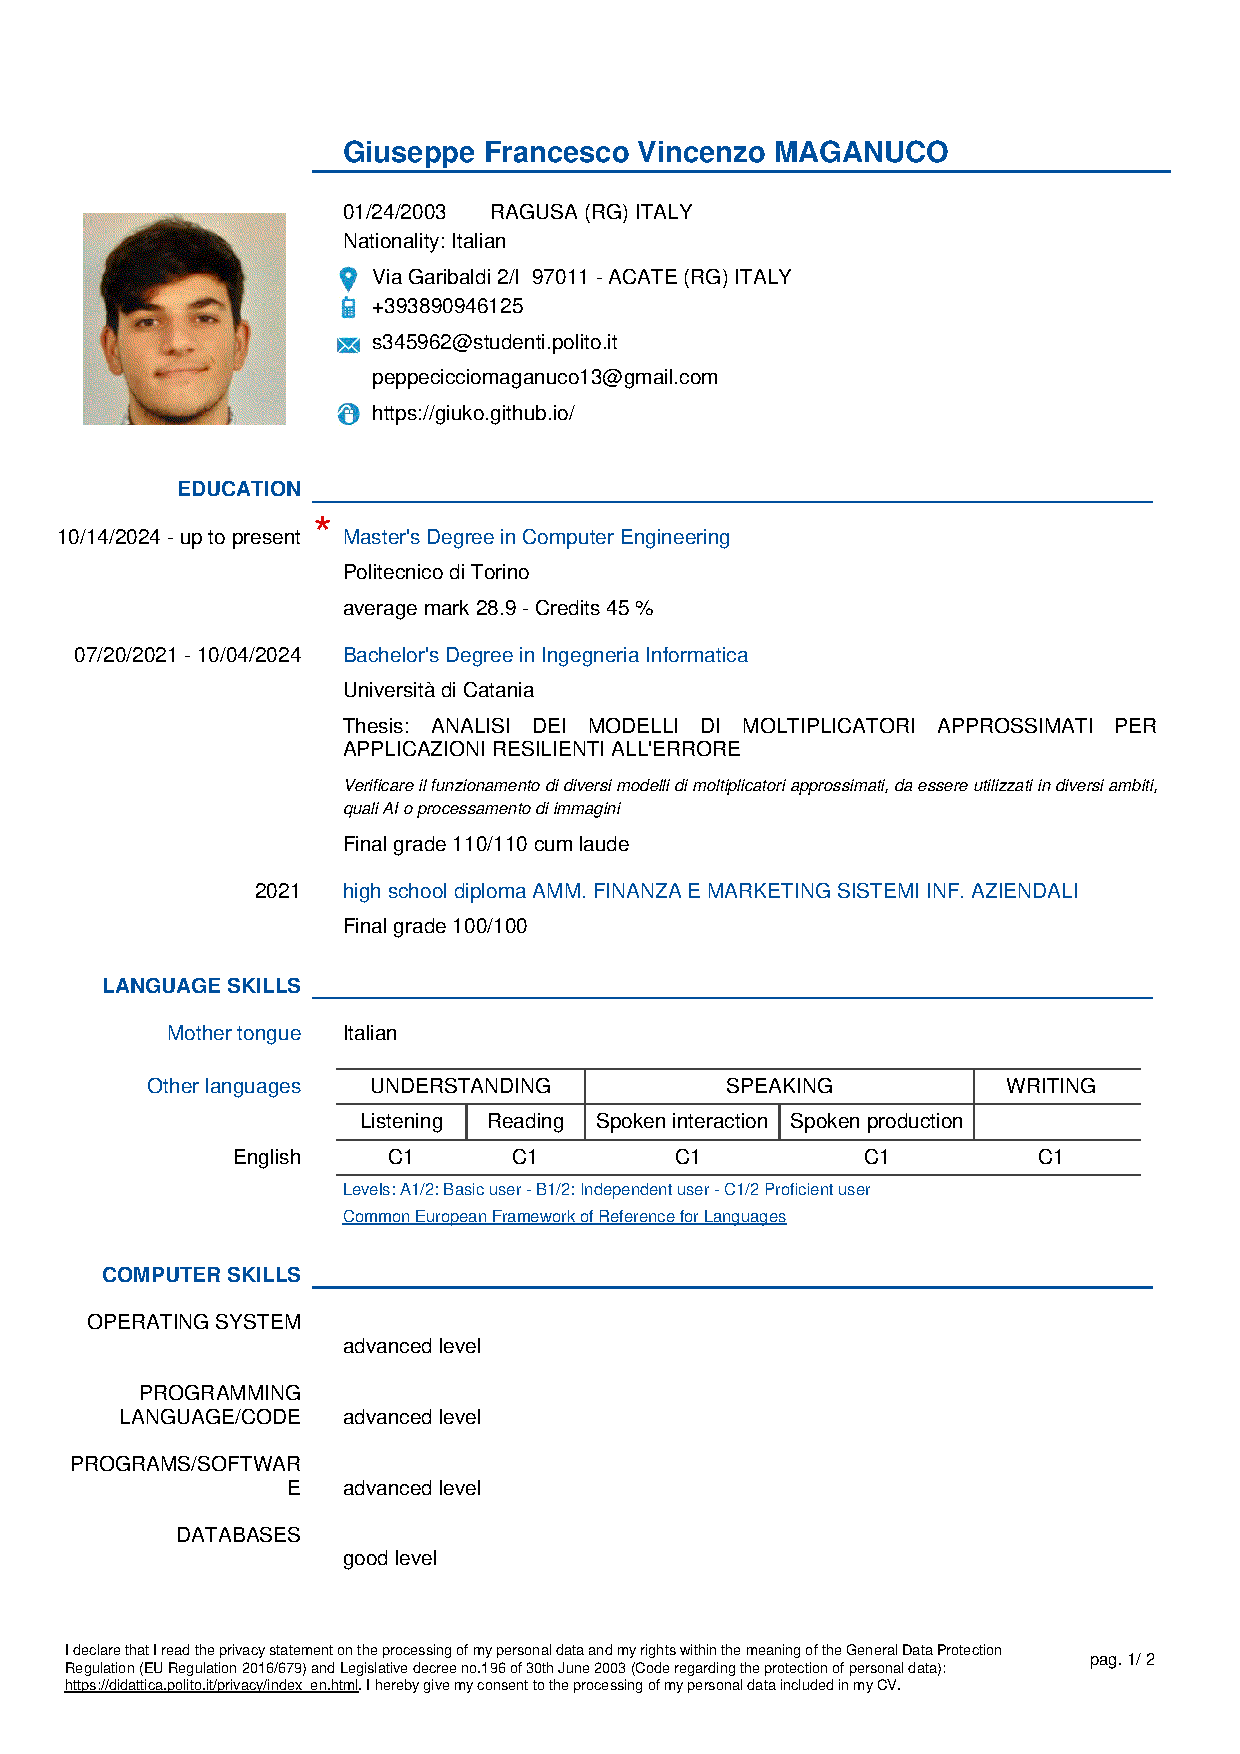
\includepdf[pages=-]{cv_polito.pdf}

\end{document}

